\section{Static Obstacle Avoidance Tests} 
In order to evaluate the behaviour of our controller when it comes to avoiding static obstacles, we have set up a set of tests using \textit{Simulink Test}. These tests have been performed on different sample scenarios at different reference speeds using the same MPC configuration as in the Path Following tests (Table \ref{tab:configuration}). In particular we have simulated 22 scenarios, similarly to the first 5 scenarios in the Path Following tests (from figure \ref{fig:StraightMap} to \ref{fig:1000mCurveMap}), considering 16 straight lines with different slopes (exploring all four quadrants) and 6 curves with different radii and directions.
The scenarios we have selected are the following:
\begin{itemize}
    \item \textbf{straight lines} with:\begin{multicols}{2} \begin{itemize}
        \item[$\diamond$] 0° slope;
        \item[$\diamond$] 20° slope;
        \item[$\diamond$] 45° slope;
        \item[$\diamond$] 70° slope;
        \item[$\diamond$] 90° slope;
        \item[$\diamond$] 110° slope;
        \item[$\diamond$] 135° slope;
        \item[$\diamond$] 160° slope;
        \item[$\diamond$] 180° slope;
        \item[$\diamond$] -20° slope;
        \item[$\diamond$] -45° slope;
        \item[$\diamond$] -70° slope;
        \item[$\diamond$] -90° slope;
        \item[$\diamond$] -110° slope;
        \item[$\diamond$] -135° slope;
        \item[$\diamond$] -160° slope.
    \end{itemize}
    \end{multicols}
    
    \item \textbf{curves} with:
    \begin{multicols}{2} \begin{itemize}
        \item[$\diamond$] 1000 $m$ radius clockwise;
        \item[$\diamond$] 500 $m$ radius clockwise;
        \item[$\diamond$] 300 $m$ radius clockwise;
        \item[$\diamond$] 300 $m$ radius counterclockwise;
        \item[$\diamond$] 500 $m$ radius counterclockwise;
        \item[$\diamond$] 1000 $m$ radius counterclockwise;
    \end{itemize}
    \end{multicols}
\end{itemize}

In the following subsections we describe in detail the test performed.

\subsection{Single Static Obstacle}
We have started off from the easiest case of obstacle avoidance possible, one static obstacle on the whole reference map. This is the easiest case possible to implement because once detected an obstacle, the controller does not need to search for another; moreover, since the obstacle is static, the controller does not need to know its speed in order to calculate its trajectory either.
In particular we have placed the obstacle always exactly in the middle of the simulated map so that the detection of the obstacle and consequent overtaking maneuver could be executed correctly by the controller in any circumstance.
Similarly to the tests performed to assert the path following task, we have performed the obstacle avoidance tests taking into account equations \ref{dynamic_equation} and \ref{eq:lateral_dev} on lateral acceleration and lateral deviation respectively, in order to monitor whether or not requirements 1 and 5 (Section \ref{System_Requirements}) on maximum lateral error and maximum lateral acceleration were satisfied.
Regarding the other requirements described in the same section, we suppose that the controller and the set of sensors installed take care of them.
Regarding requirements 1 and 5, tests are considered passed if the following conditions are verified:
\begin{itemize}
    \item lateral deviation always greater than or equal to 2 $m$ and lower than or equal to 6 $m$ when performing the overtaking maneuver;
    \item  lateral deviation must not exceed 5 $m$ and be lower than 3 $m$ for more than 1 $s$ when performing the overtaking maneuver; 
    \item lateral deviation lower than 6 $m$ at any point of time;
    \item lateral acceleration does not exceed 2.0 $m/s^2$ for more than 0.5 $s$ at any point of time.
\end{itemize}
We have chosen those limits because we assumed that a lane is 4 $m$ wide and a lateral deviation of 0 $m$ means that we are exactly on the reference trajectory, always considered to be on the right lane. The 2 $m$ bound represents, instead, the boundary between the right and the left lane while the upper bound of 6 $m$ is the leftest boundary of the left lane.
In order to verify these conditions, we have set up a test bench to monitor them.
Details about the single static obstacle avoidance tests performed can be found in the documents included in the repository\footnote{The ``Single\_Static\_Obstacle\_Avoidance-Test\_Report" and ``Single\_Static\_Obstacle\_Avoidance-Test\_Specification\_Report" files generated by Simulink Test are included in the /Documentation/Test Reports/ file path.}.\\
Performing the tests we have noticed that our controller performs very well at medium/low speeds (such as 40-50 km/h) while it has some stability issues at lower speeds. The figures below show a comparison between the overtaking maneuver performed respectively at 50 km/h (Figure \ref{fig:overtaking_50}) and at 10 km/h (Figure \ref{fig:overtaking_10}), highlighting how the performance of the MPC degrades with lower speeds.

\begin{figure}[H]
    \centering
   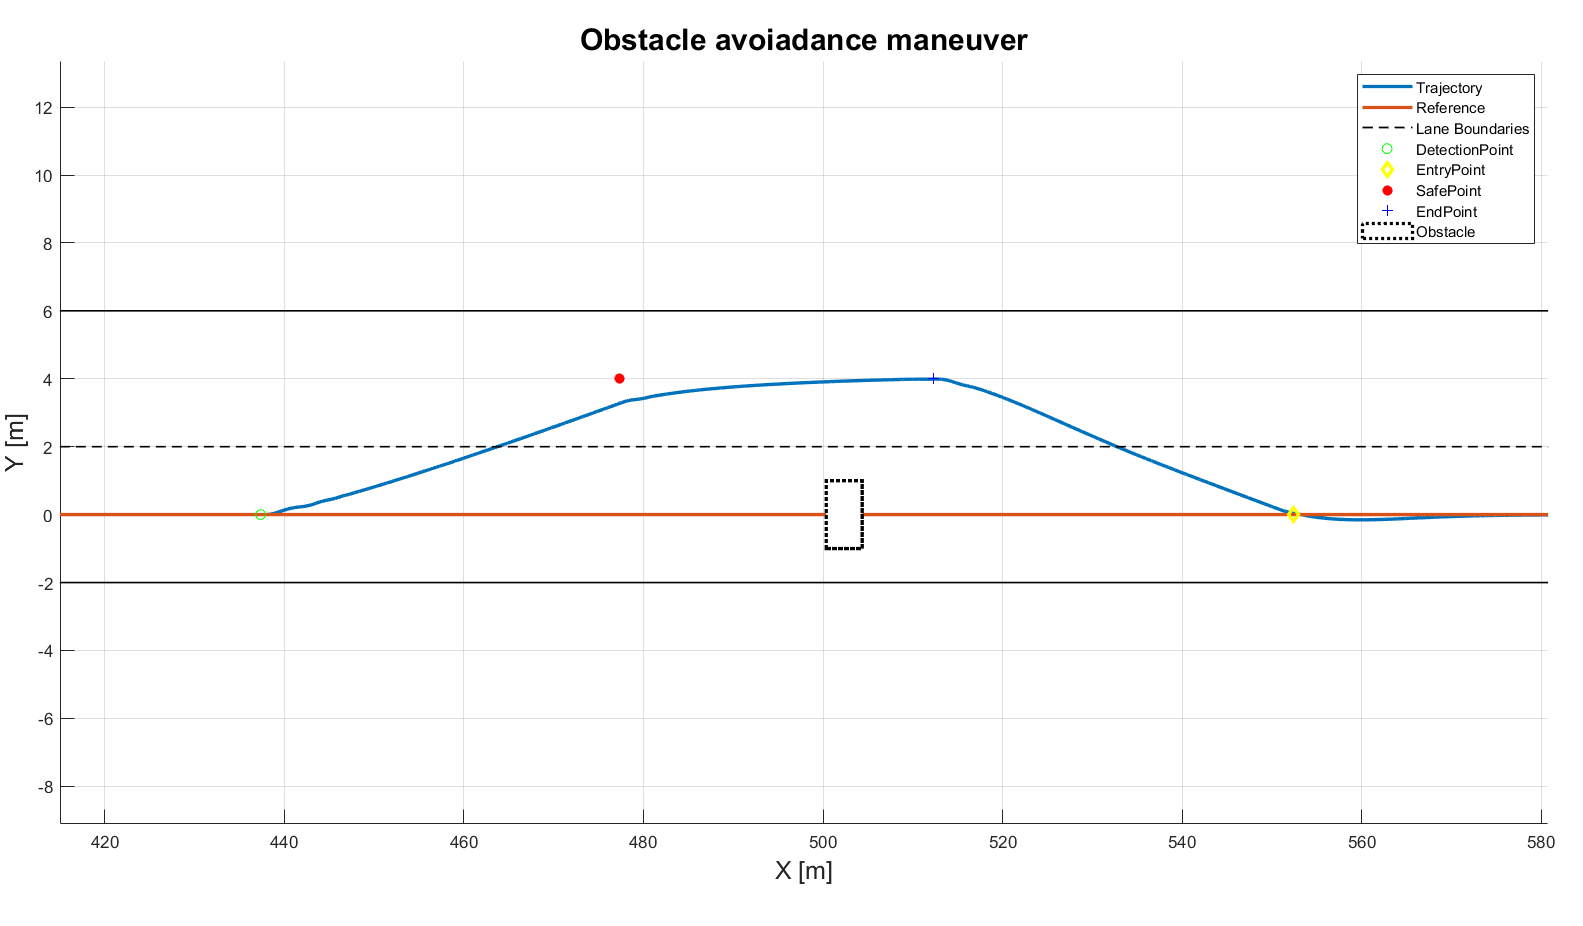
\includegraphics[width=1\textwidth,keepaspectratio]{Figures/StaticAvoidance1.png}
    \caption{Overtaking maneuver at 50 km/h}
    \label{fig:overtaking_50}
\end{figure}

\begin{figure}[H]
    \centering
    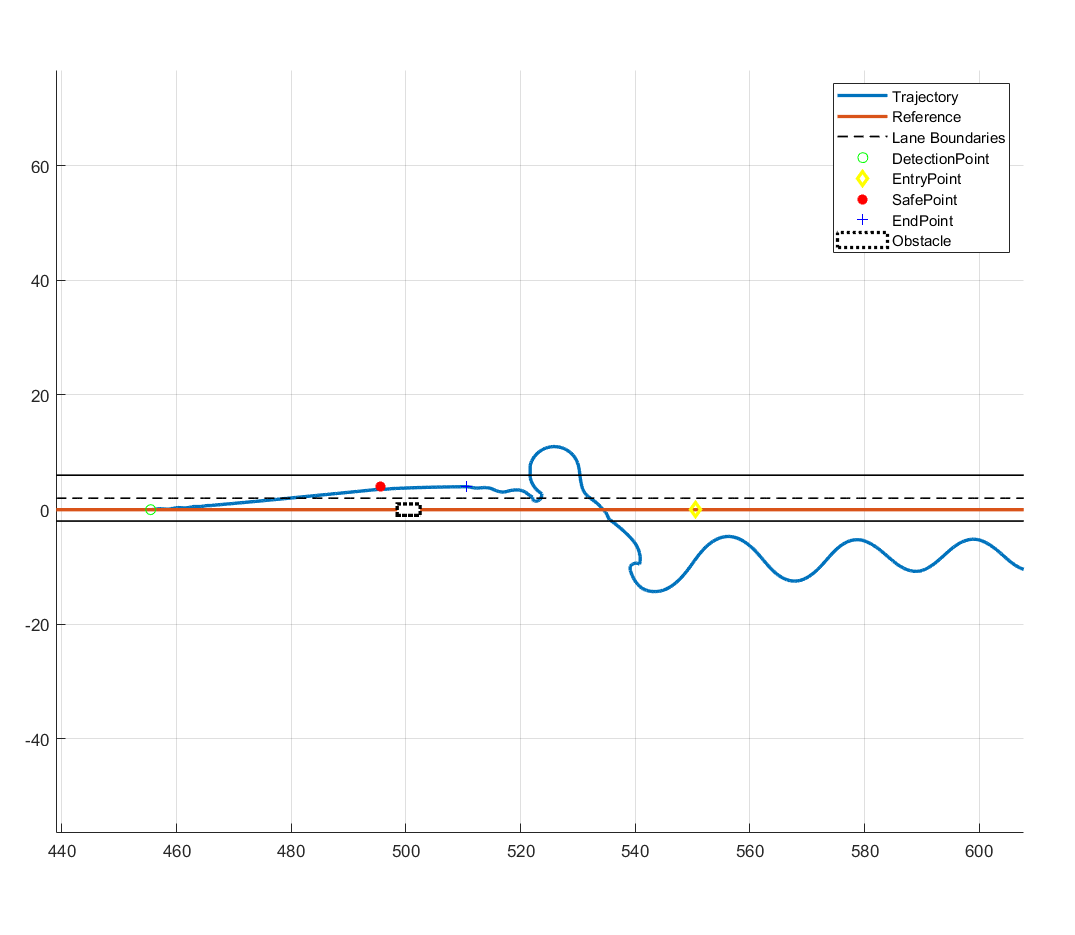
\includegraphics[width=1\textwidth,keepaspectratio]{Figures/Failed10kmh.png}
    \caption{Overtaking maneuver at 10 km/h}
    \label{fig:overtaking_10}
\end{figure}




The tests have also highlighted how the performance of our MPC is still fairly good at higher speeds (such as 100 km/h) with some issues only on the curved scenarios with curvature radius of 300 $m$ when the vehicle travels counterclockwise. \\ 
More details about the failed tests and the subsequent considerations are reported in the next subsection.

\subsection{Failed test analysis and important considerations} \label{subsection:failed_tests}
The ``Single\_Static\_Obstacle\_Avoidance-Test\_Report" shows all the issues that have arisen during the testing phase. In this section we describe the most important ones and we make some considerations.
As shown in Figure \ref{fig:fail100kmh}, our controller is not fully able to be compliant with the first condition described in the previous subsection when we are travelling at 100 km/h on a curve with 300 $m$ radius with counterclockwise direction. In this case, the ego vehicle is not able to perform in time the overtaking maneuver because of the high speed. 

\begin{figure}[H]
    \centering
    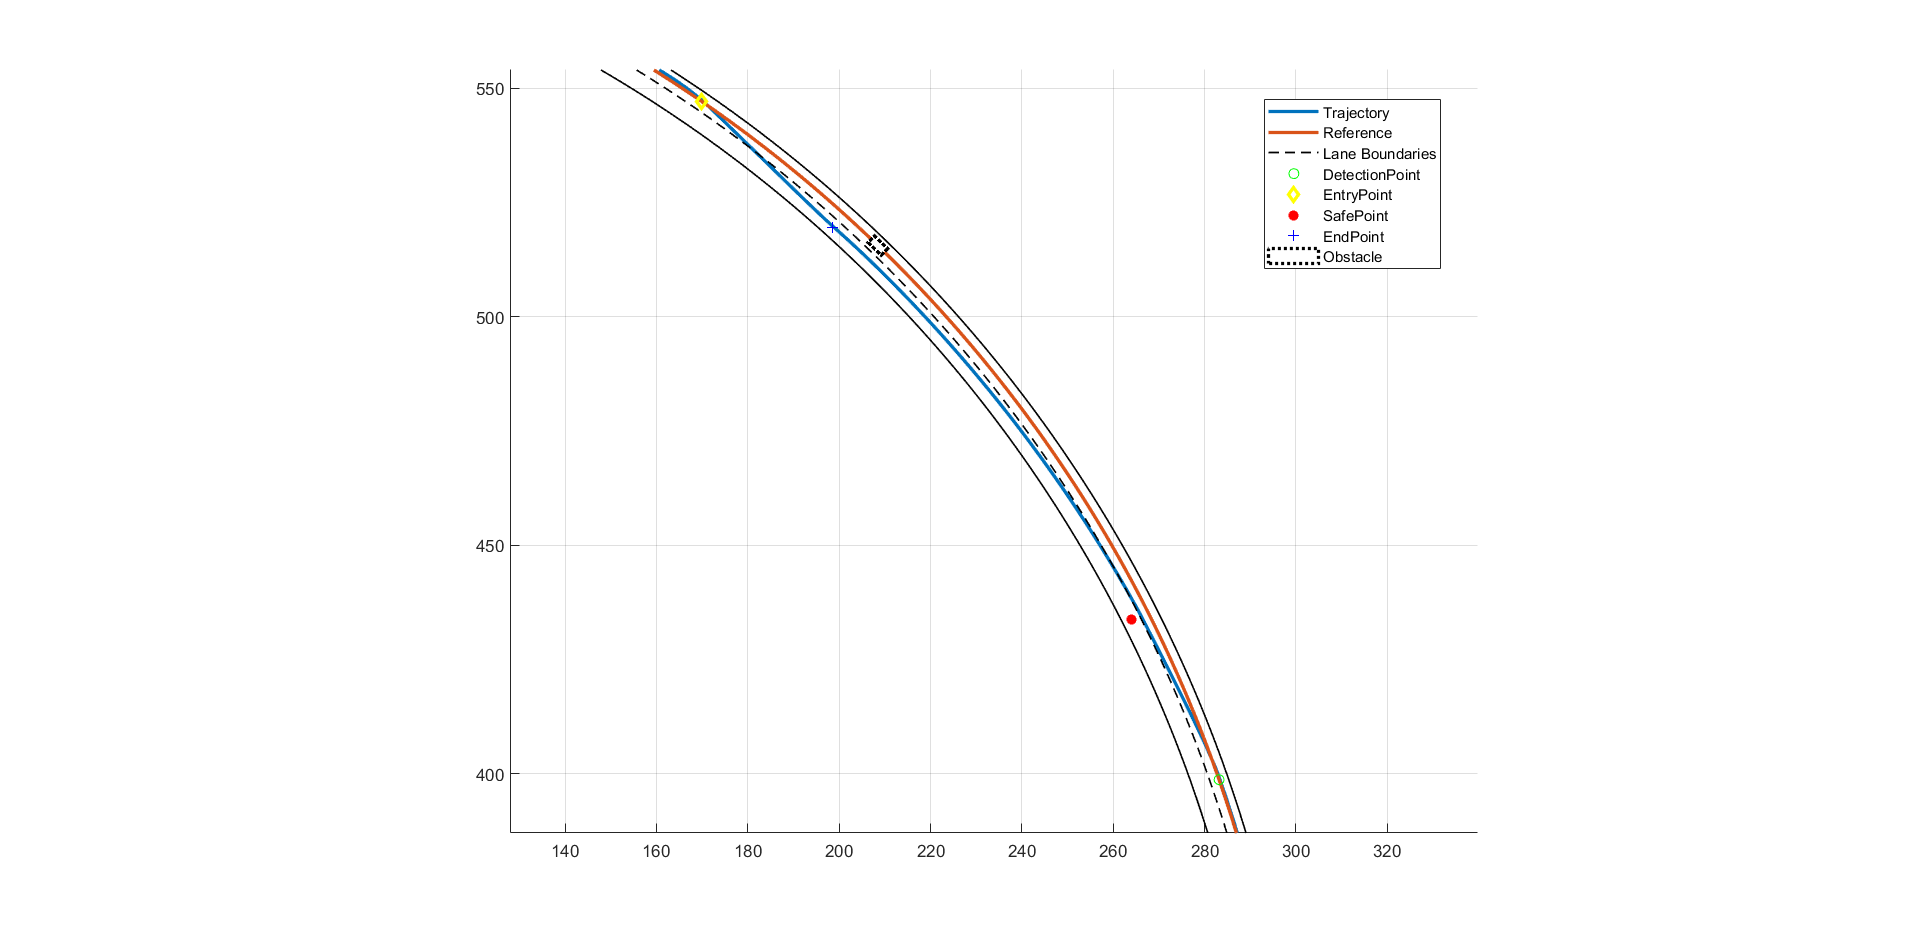
\includegraphics[width=1.1\textwidth,keepaspectratio]{Figures/fail100kmh.png}
    \caption{Failure during the overtaking maneuver at 100 km/h on a curve with 300 $m$ wide radius with counterclockwise direction }
    \label{fig:fail100kmh}
\end{figure}
Despite this anomaly, we recognize that this is not a major problem since breaking this particular assessment does not fully compromise the ability of the controller to avoid the obstacle since, at this reference speed, the safety distance is 100 $m$ and so, going slightly over the so-called ``\textit{SafePoint}", does not represent a dangerous situation. Moreover, it only occurs on curves with quite small radius when the vehicle is steering towards the left side.\\


The main issue we have found is that our controller is not able to perform a proper overtaking maneuver at low speed. Critical speeds range from 10 to about 30 km/h. An example of this behaviour on a curved scenario is shown in Figure \ref{fig:controller_madness}.
\begin{figure}[H]
    \centering
    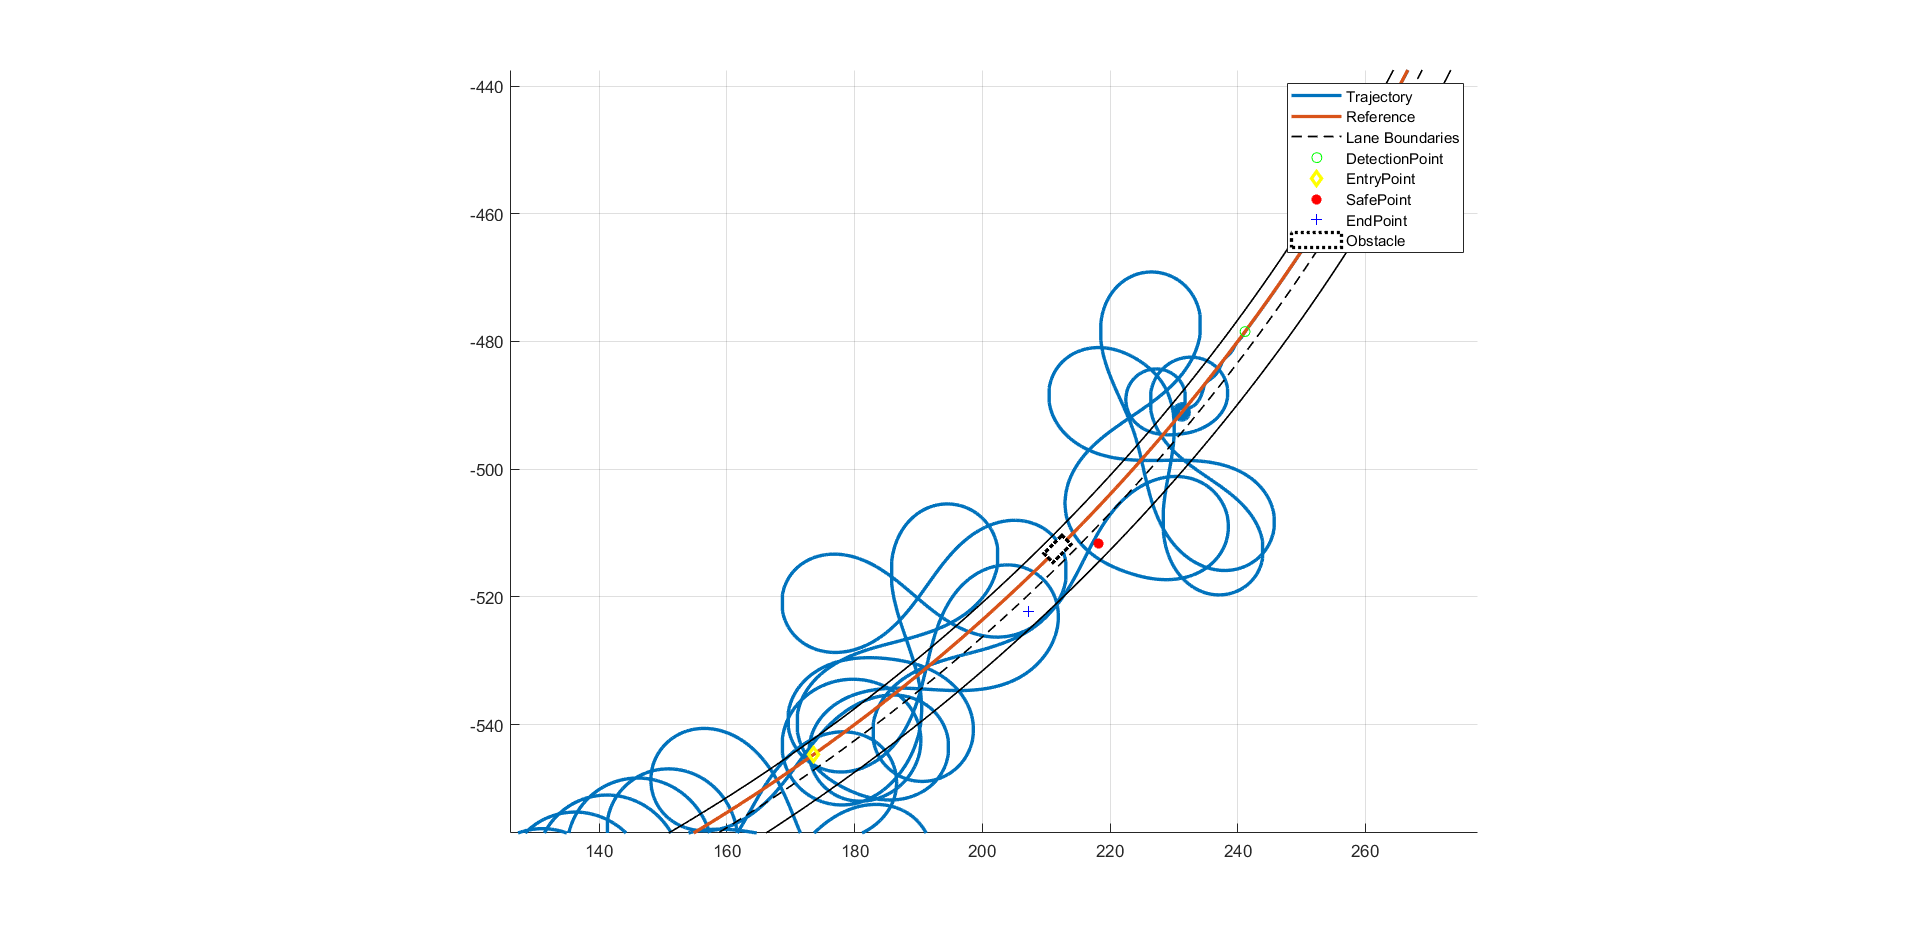
\includegraphics[width=1\textwidth,keepaspectratio]{Figures/Failed300m10kmh.png}
    \caption{Example of controller stability issues at 10 km/h}
    \label{fig:controller_madness}
\end{figure}

As you might guess, this issue implies that we are no longer able to comply with the sixth requirement we imposed in the starting phase of our project described in Section \ref{System_Requirements}.
Having based the development of our whole project on the V-model, as already stated in the Introduction of this report, going back to fix this issue in order to make the MPC work properly at low speeds would imply modifying the weights in the weights function and repeating all the testing phases.
We have decided to do so only for a certain speed range which means that we are actually implementing a new MPC with different weights in order to manage this speed range while keeping the current configuration for the set of speeds already tested on which our MPC has been already validated.
This decision implies a higher modularity of our project, that from now on will be based on two sub-problems, consisting of two different speed ranges which will be managed by two different MPCs: 
\begin{itemize}
    \item the current MPC which will manage speeds ranging from 40 km/h to 100 km/h;
    \item a new MPC which will be developed to be in charge for speeds in the range from 10 km/h to 40 km/h.
\end{itemize}

We believe that this is the optimal solution in order to be able to continue the tests on the current MPC, considering those already performed as valid in the proper speed range and to have a faster validation phase for the second MPC that will be developed afterwards.


\subsection{Multiple Static Obstacles}
